\documentclass[12pt, aspectratio=169]{beamer} % options: handout

\usetheme{metropolis}
\setbeamertemplate{frame footer}{\insertshorttitle~| \insertsection}
\setbeamerfont{page number in head/foot}{size=\tiny}
\setbeamercolor{footline}{fg=gray}

\usepackage[greek, czech]{babel}
\usepackage[T1]{fontenc}
\usepackage{amssymb}
\usepackage{amsmath}
\usepackage{amssymb}

\metroset{sectionpage=none} % schova stranky s nazvem sekce

\title[Optimalizace FVE]{Optimalizace investičních prostředků z hlediska výnosu fotovoltaických elektráren}
\author[Kotlan]{Petr Kotlan\\ Vedoucí práce: Ing. Roman Vaibar, Ph.D., MBA}
\institute[Přf UJEP]{Přírodovědecká fakulta\\ Univerzita J. E. Purkyně}
\date{}

\begin{document}


\begin{frame}[plain]

    \maketitle
    
\end{frame}

\section{Anotace}

\begin{frame}{\insertsection}
Cílem bakalářské práce je vyvinout aplikaci, která pomocí lineárního programování
optimalizuje rozdělení investičních prostředků pro instalaci fotovoltaických elektráren na daných objektech.
Optimalizace bude provedena na základě následujících hledisek:

\begin{itemize}
    \item typu střechy -- rovná, sedlová, valbová atd.,
    \item spotřeby v daném místě,
    \item ceny energie definované odkupem dle spotových cen OTE, a.s.,
    \item optimalizace uložiště,
    \item výpočtu předpokládaného ročního výkonu dle osvitových hodin.
\end{itemize}

\end{frame}

\section{Osnova}

\begin{frame}{\insertsection}
    \begin{enumerate}
        \item Úvod
        \item Současné modely výnosů fotovoltaických elektráren v ČR
        \item Teoretická část
        \begin{itemize}
            \item Přehled ekonomických pojmů
            \item Základní modely matematické optimalizace
        \end{itemize}
        \item Praktická část
        \begin{itemize}
            \item Popis aplikace
            \item Případové studie
        \end{itemize}
        \item Zhodnocení výsledků
        \item Závěr
        
    \end{enumerate}
\end{frame}


\section{Datové zdroje a uložiště}

\begin{frame}{\insertsection}
    \begin{block}{Zdroje}
        \begin{itemize}
            \item \href{https://www.ote-cr.cz/}{OTE, a.s.},
            \item FVE DCUK API (rozhraní pro správu FVE projektů),
            \item \href{https://www.mesec.cz/produkty/sporici-ucty/}{srovnání spořících účtů}
            \item \href{https://www.chmi.cz/historicka-data/pocasi/denni-data/Denni-data-dle-z.-123-1998-Sb}{ČHMÚ -- denní úhrn doby trvání slunečního svitu}
        \end{itemize}        
    \end{block}
    \begin{block}{Uložiště}
        \begin{itemize}
            \item InfluxDB
            \item MariaDB
        \end{itemize}
    \end{block}
\end{frame}

\section{Diagram}

\begin{frame}[standout]
    \centering
    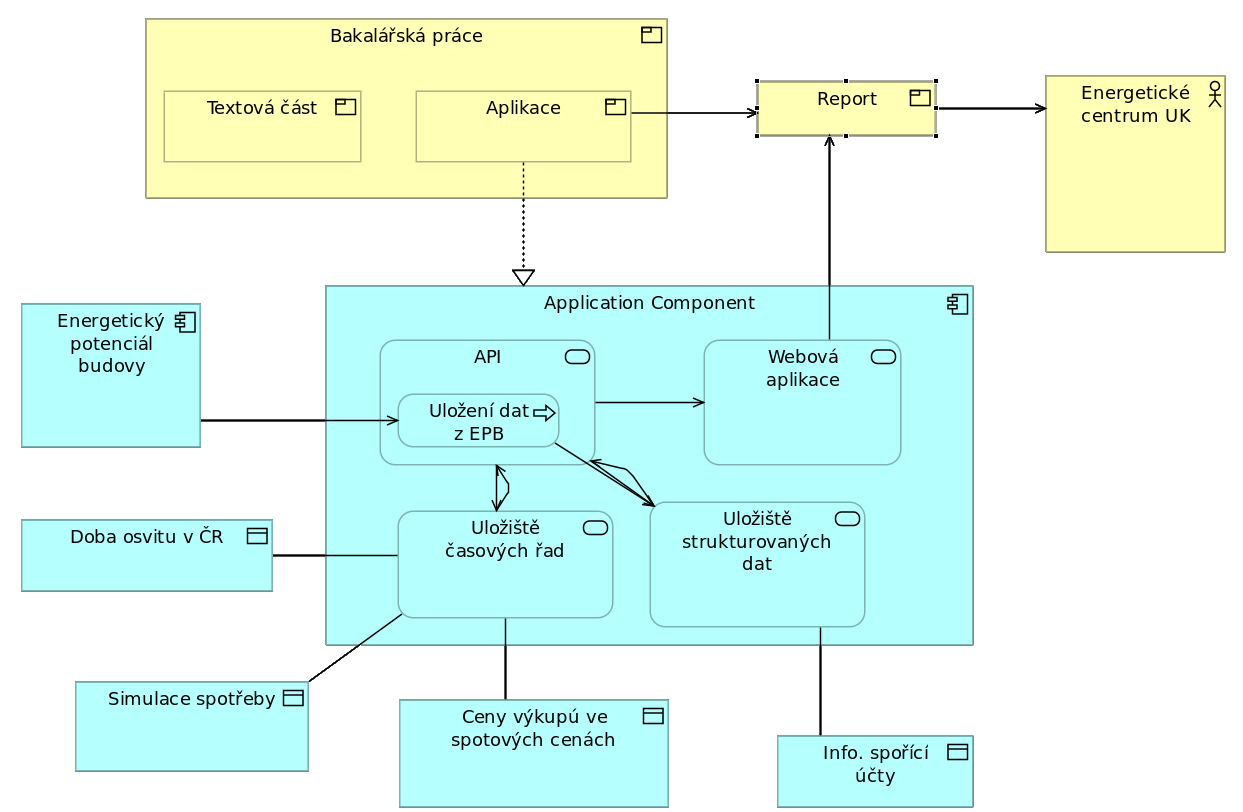
\includegraphics[height=1.1\textheight]{diagram.png}
\end{frame}

\section{Vyhodnocení výnosnosti investice}

\begin{frame}{\insertsection}
    \begin{block}{Čistá současná hodnota (NPV)}
        \vspace{10pt}
        \centering
        $NPV = \frac{P_1}{(1+i)} + \frac{P_2}{(1+i)^2} + \ldots + \frac{P_n}{(1+i)^n} - K$
    \end{block}

    \begin{block}{Vnitřní výnosové procento (IRR)}
        \vspace{10pt}
        \centering
        $\frac{P_1}{(1+IRR)} + \frac{P_2}{(1+IRR)^2} + \ldots + \frac{P_n}{(1+IRR)^n} = K$
    \end{block}
    \begin{itemize}
        \item $n$ = počet let
        \item $P_1, P_2, \ldots, P_n$ = peněžní příjmy z investice v jednotlivých letech
        \item $K$ = kapitálový výdaj
        \item $i$ = požadovaná míra výnosnosti
    \end{itemize}
\end{frame}


\section{Matematická optimalizace}

\begin{frame}{\insertsection}
    \begin{block}{Formulace úlohy}
        \vspace{10pt}
        \centering
        max $\rightarrow z = c_1x_1 + c_2x_2 + \ldots + c_nx_n$
        \break
        $Ax \leq b$
        \break
        $x \geq 0$
    \end{block}
    \begin{itemize}
        \item $x_1, x_2, \ldots, x_n$ = rozhodovací proměnné
        \item $c_1, c_2, \ldots, c_n$ = cenové koeficienty
        \item $A$ = matice strukturních koeficientů
        \item $b$ = požadavková čísla
        \item $z$ = cílová funkce
    \end{itemize}

\end{frame}

\section{Dalsi postup}

\end{document}